\section{INTRODUCTION}
Facial expression recognition (FER) is the automated process of identifying and categorizing facial expressions in images or videos. This task involves interpreting emotions such as happiness, sadness, anger, surprise, disgust, and fear based on facial features. FER has become essential in human-computer interaction, enabling systems to understand and respond to human emotions, enhancing user experience across diverse applications, including virtual assistants, gaming, and social robotics.

While facial expressions are a primary modality for conveying emotions, other factors such as body movements, voice, and physiological signals also play a role in emotion recognition. Despite these, FER remains one of the most widely researched and applied aspects of non-verbal communication in affective computing due to its relative ease of acquisition and analysis.

The nature of FER datasets is pivotal to the advancement of this field. Datasets differ based on annotation types and data acquisition methods. Early works, such as Ekman’s categorical model \cite{Ekman}, proposed six basic emotions (anger, surprise, happiness, fear, sadness, and disgust), asserting that these emotions are universally recognized across cultures. However, recent psychological research suggests that emotional expressions can vary in intensity and frequency across different cultures, challenging the universality of categorical models \cite{not_culturally_universal}. To address this, alternative annotation models, such as the \textbf{Facial Action Coding System} (\textbf{FACS}), have been introduced. FACS, in particular, breaks down facial expressions into muscle movements called Action Units (AUs), offering a more granular representation of expressions and their physical manifestations. This approach is valuable for cross-cultural analysis, as it focuses on the mechanical aspects of facial movement rather than subjective emotional experience\cite{FACS0}.

Datasets also differ in terms of the type of data collected—whether \textbf{static} or \textbf{dynamic}, \textbf{posed} or \textbf{spontaneous}, \textbf{2D} or \textbf{3D}, and acquired in controlled \textbf{laboratory settings} or \textbf{in-the-wild }environments. Static datasets consist of single images capturing spatial information, while dynamic datasets capture temporal evolution, allowing for the extraction of both spatial and temporal features. The latter is particularly useful for understanding the subtleties of expressions over time. Posed datasets, where subjects are instructed to display specific expressions, are easier to collect but may not reflect real-world scenarios. Conversely, spontaneous datasets contain naturally occurring expressions, which are more representative of real-life emotions but are more expensive and challenging to collect. Figure \ref{datasets_examples} provides an example of some common FER datasets, highlighting their characteristics.


\begin{figure*}
	\centering
	\begin{subfigure}{0.2\textwidth}
		
\includegraphics[width=\linewidth]{images/CK_happy.png}
		\caption{}
		\label{fig:subfigA}
	\end{subfigure}
   \hspace{0.15cm}
	\begin{subfigure}{0.2\textwidth}
        
\includegraphics[width=\linewidth]{images/AffectNet.jpg}
		\caption{}
		\label{fig:subfigB}
	\end{subfigure}
   \hspace{0.1cm}
	\begin{subfigure}{0.45\textwidth}
        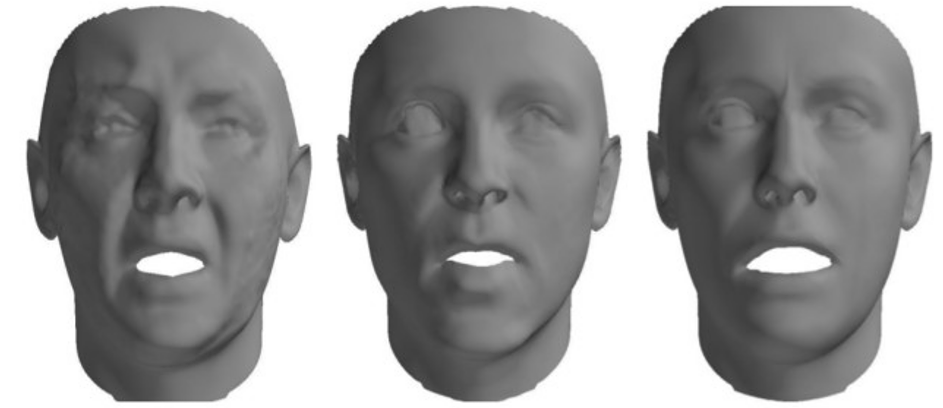
\includegraphics[width=\linewidth]{images/4DFAB_3D.png}
	        \caption{}
	        \label{fig:subfigC}
         \end{subfigure}
         \caption{FER datasets examples - (a) CK+\protect\cite{CK+} sample (grayscale, static, posed, lab acquired), (b) AffectNet\protect\cite{AffectNet} sample (RGB, static, spontaneous), (c) 4DFAB\protect\cite{4DFAB} sample (3D mesh, dynamic, spontaneous, lab)}
    \label{datasets_examples}
\end{figure*}

The selection of a dataset has a significant impact on the performance and generalizability of FER models. Moreover, the integration of multimodal data, including audio and physiological signals, enhances model robustness, especially in dynamic datasets, by providing complementary information for emotion recognition. The increasing use of 3D representations, such as depth maps and point clouds, also helps mitigate challenges like illumination variation and occlusion, though they come at a higher cost compared to 2D representations.

As FER continues to evolve, the demand for datasets that better reflect the diversity and complexity of human emotion is growing. The global emotion recognition market, valued at $21.7$ billion in 2021, is projected to reach $136.2$ billion by 2031, with a compound annual growth rate (CAGR) of 20.5\% \cite{Allied-market-research}, underscoring the expanding interest and applications of FER technology across industries.




